% Generated by Sphinx.
\def\sphinxdocclass{report}
\documentclass[letterpaper,10pt,english]{sphinxmanual}
\usepackage[utf8]{inputenc}
\DeclareUnicodeCharacter{00A0}{\nobreakspace}
\usepackage[T1]{fontenc}
\usepackage{babel}
\usepackage{times}
\usepackage[Bjarne]{fncychap}
\usepackage{longtable}
\usepackage{sphinx}


\title{ROACHNEST Documentation}
\date{December 13, 2011}
\release{1}
\author{Danny Price}
\newcommand{\sphinxlogo}{}
\renewcommand{\releasename}{Release}
\makeindex

\makeatletter
\def\PYG@reset{\let\PYG@it=\relax \let\PYG@bf=\relax%
    \let\PYG@ul=\relax \let\PYG@tc=\relax%
    \let\PYG@bc=\relax \let\PYG@ff=\relax}
\def\PYG@tok#1{\csname PYG@tok@#1\endcsname}
\def\PYG@toks#1+{\ifx\relax#1\empty\else%
    \PYG@tok{#1}\expandafter\PYG@toks\fi}
\def\PYG@do#1{\PYG@bc{\PYG@tc{\PYG@ul{%
    \PYG@it{\PYG@bf{\PYG@ff{#1}}}}}}}
\def\PYG#1#2{\PYG@reset\PYG@toks#1+\relax+\PYG@do{#2}}

\def\PYG@tok@gd{\def\PYG@tc##1{\textcolor[rgb]{0.63,0.00,0.00}{##1}}}
\def\PYG@tok@gu{\let\PYG@bf=\textbf\def\PYG@tc##1{\textcolor[rgb]{0.50,0.00,0.50}{##1}}}
\def\PYG@tok@gt{\def\PYG@tc##1{\textcolor[rgb]{0.00,0.25,0.82}{##1}}}
\def\PYG@tok@gs{\let\PYG@bf=\textbf}
\def\PYG@tok@gr{\def\PYG@tc##1{\textcolor[rgb]{1.00,0.00,0.00}{##1}}}
\def\PYG@tok@cm{\let\PYG@it=\textit\def\PYG@tc##1{\textcolor[rgb]{0.25,0.50,0.56}{##1}}}
\def\PYG@tok@vg{\def\PYG@tc##1{\textcolor[rgb]{0.73,0.38,0.84}{##1}}}
\def\PYG@tok@m{\def\PYG@tc##1{\textcolor[rgb]{0.13,0.50,0.31}{##1}}}
\def\PYG@tok@mh{\def\PYG@tc##1{\textcolor[rgb]{0.13,0.50,0.31}{##1}}}
\def\PYG@tok@cs{\def\PYG@tc##1{\textcolor[rgb]{0.25,0.50,0.56}{##1}}\def\PYG@bc##1{\colorbox[rgb]{1.00,0.94,0.94}{##1}}}
\def\PYG@tok@ge{\let\PYG@it=\textit}
\def\PYG@tok@vc{\def\PYG@tc##1{\textcolor[rgb]{0.73,0.38,0.84}{##1}}}
\def\PYG@tok@il{\def\PYG@tc##1{\textcolor[rgb]{0.13,0.50,0.31}{##1}}}
\def\PYG@tok@go{\def\PYG@tc##1{\textcolor[rgb]{0.19,0.19,0.19}{##1}}}
\def\PYG@tok@cp{\def\PYG@tc##1{\textcolor[rgb]{0.00,0.44,0.13}{##1}}}
\def\PYG@tok@gi{\def\PYG@tc##1{\textcolor[rgb]{0.00,0.63,0.00}{##1}}}
\def\PYG@tok@gh{\let\PYG@bf=\textbf\def\PYG@tc##1{\textcolor[rgb]{0.00,0.00,0.50}{##1}}}
\def\PYG@tok@ni{\let\PYG@bf=\textbf\def\PYG@tc##1{\textcolor[rgb]{0.84,0.33,0.22}{##1}}}
\def\PYG@tok@nl{\let\PYG@bf=\textbf\def\PYG@tc##1{\textcolor[rgb]{0.00,0.13,0.44}{##1}}}
\def\PYG@tok@nn{\let\PYG@bf=\textbf\def\PYG@tc##1{\textcolor[rgb]{0.05,0.52,0.71}{##1}}}
\def\PYG@tok@no{\def\PYG@tc##1{\textcolor[rgb]{0.38,0.68,0.84}{##1}}}
\def\PYG@tok@na{\def\PYG@tc##1{\textcolor[rgb]{0.25,0.44,0.63}{##1}}}
\def\PYG@tok@nb{\def\PYG@tc##1{\textcolor[rgb]{0.00,0.44,0.13}{##1}}}
\def\PYG@tok@nc{\let\PYG@bf=\textbf\def\PYG@tc##1{\textcolor[rgb]{0.05,0.52,0.71}{##1}}}
\def\PYG@tok@nd{\let\PYG@bf=\textbf\def\PYG@tc##1{\textcolor[rgb]{0.33,0.33,0.33}{##1}}}
\def\PYG@tok@ne{\def\PYG@tc##1{\textcolor[rgb]{0.00,0.44,0.13}{##1}}}
\def\PYG@tok@nf{\def\PYG@tc##1{\textcolor[rgb]{0.02,0.16,0.49}{##1}}}
\def\PYG@tok@si{\let\PYG@it=\textit\def\PYG@tc##1{\textcolor[rgb]{0.44,0.63,0.82}{##1}}}
\def\PYG@tok@s2{\def\PYG@tc##1{\textcolor[rgb]{0.25,0.44,0.63}{##1}}}
\def\PYG@tok@vi{\def\PYG@tc##1{\textcolor[rgb]{0.73,0.38,0.84}{##1}}}
\def\PYG@tok@nt{\let\PYG@bf=\textbf\def\PYG@tc##1{\textcolor[rgb]{0.02,0.16,0.45}{##1}}}
\def\PYG@tok@nv{\def\PYG@tc##1{\textcolor[rgb]{0.73,0.38,0.84}{##1}}}
\def\PYG@tok@s1{\def\PYG@tc##1{\textcolor[rgb]{0.25,0.44,0.63}{##1}}}
\def\PYG@tok@gp{\let\PYG@bf=\textbf\def\PYG@tc##1{\textcolor[rgb]{0.78,0.36,0.04}{##1}}}
\def\PYG@tok@sh{\def\PYG@tc##1{\textcolor[rgb]{0.25,0.44,0.63}{##1}}}
\def\PYG@tok@ow{\let\PYG@bf=\textbf\def\PYG@tc##1{\textcolor[rgb]{0.00,0.44,0.13}{##1}}}
\def\PYG@tok@sx{\def\PYG@tc##1{\textcolor[rgb]{0.78,0.36,0.04}{##1}}}
\def\PYG@tok@bp{\def\PYG@tc##1{\textcolor[rgb]{0.00,0.44,0.13}{##1}}}
\def\PYG@tok@c1{\let\PYG@it=\textit\def\PYG@tc##1{\textcolor[rgb]{0.25,0.50,0.56}{##1}}}
\def\PYG@tok@kc{\let\PYG@bf=\textbf\def\PYG@tc##1{\textcolor[rgb]{0.00,0.44,0.13}{##1}}}
\def\PYG@tok@c{\let\PYG@it=\textit\def\PYG@tc##1{\textcolor[rgb]{0.25,0.50,0.56}{##1}}}
\def\PYG@tok@mf{\def\PYG@tc##1{\textcolor[rgb]{0.13,0.50,0.31}{##1}}}
\def\PYG@tok@err{\def\PYG@bc##1{\fcolorbox[rgb]{1.00,0.00,0.00}{1,1,1}{##1}}}
\def\PYG@tok@kd{\let\PYG@bf=\textbf\def\PYG@tc##1{\textcolor[rgb]{0.00,0.44,0.13}{##1}}}
\def\PYG@tok@ss{\def\PYG@tc##1{\textcolor[rgb]{0.32,0.47,0.09}{##1}}}
\def\PYG@tok@sr{\def\PYG@tc##1{\textcolor[rgb]{0.14,0.33,0.53}{##1}}}
\def\PYG@tok@mo{\def\PYG@tc##1{\textcolor[rgb]{0.13,0.50,0.31}{##1}}}
\def\PYG@tok@mi{\def\PYG@tc##1{\textcolor[rgb]{0.13,0.50,0.31}{##1}}}
\def\PYG@tok@kn{\let\PYG@bf=\textbf\def\PYG@tc##1{\textcolor[rgb]{0.00,0.44,0.13}{##1}}}
\def\PYG@tok@o{\def\PYG@tc##1{\textcolor[rgb]{0.40,0.40,0.40}{##1}}}
\def\PYG@tok@kr{\let\PYG@bf=\textbf\def\PYG@tc##1{\textcolor[rgb]{0.00,0.44,0.13}{##1}}}
\def\PYG@tok@s{\def\PYG@tc##1{\textcolor[rgb]{0.25,0.44,0.63}{##1}}}
\def\PYG@tok@kp{\def\PYG@tc##1{\textcolor[rgb]{0.00,0.44,0.13}{##1}}}
\def\PYG@tok@w{\def\PYG@tc##1{\textcolor[rgb]{0.73,0.73,0.73}{##1}}}
\def\PYG@tok@kt{\def\PYG@tc##1{\textcolor[rgb]{0.56,0.13,0.00}{##1}}}
\def\PYG@tok@sc{\def\PYG@tc##1{\textcolor[rgb]{0.25,0.44,0.63}{##1}}}
\def\PYG@tok@sb{\def\PYG@tc##1{\textcolor[rgb]{0.25,0.44,0.63}{##1}}}
\def\PYG@tok@k{\let\PYG@bf=\textbf\def\PYG@tc##1{\textcolor[rgb]{0.00,0.44,0.13}{##1}}}
\def\PYG@tok@se{\let\PYG@bf=\textbf\def\PYG@tc##1{\textcolor[rgb]{0.25,0.44,0.63}{##1}}}
\def\PYG@tok@sd{\let\PYG@it=\textit\def\PYG@tc##1{\textcolor[rgb]{0.25,0.44,0.63}{##1}}}

\def\PYGZbs{\char`\\}
\def\PYGZus{\char`\_}
\def\PYGZob{\char`\{}
\def\PYGZcb{\char`\}}
\def\PYGZca{\char`\^}
\def\PYGZsh{\char`\#}
\def\PYGZpc{\char`\%}
\def\PYGZdl{\char`\$}
\def\PYGZti{\char`\~}
% for compatibility with earlier versions
\def\PYGZat{@}
\def\PYGZlb{[}
\def\PYGZrb{]}
\makeatother

\begin{document}

\maketitle
\tableofcontents
\phantomsection\label{index::doc}



\chapter{Copyright \& Licensing}
\label{index:roachnest-documentation}\label{index:copyright-licensing}
\textbf{ROACHNEST: A browser based user interface for monitor \& control of CASPER hardware}

\emph{Copyright (C) 2011  Danny Price}

\textbf{Everything I've written:} GNU General Public License (GPL)

This program is free software: you can redistribute it and/or modify
it under the terms of the GNU General Public License as published by
the Free Software Foundation, either version 3 of the License, or
(at your option) any later version.

This program is distributed in the hope that it will be useful,
but WITHOUT ANY WARRANTY; without even the implied warranty of
MERCHANTABILITY or FITNESS FOR A PARTICULAR PURPOSE.  See the
GNU General Public License for more details.

You should have received a copy of the GNU General Public License
along with this program.  If not, see \textless{}\href{http://www.gnu.org/licenses/}{http://www.gnu.org/licenses/}\textgreater{}

\textbf{Everything else:} As per author's original licensing terms.
Bottle.py and Flot are MIT licensed, Blueprint is a modified MIT license,
sqlite3 is public domain.


\chapter{Introduction}
\label{index:introduction}
Roachnest is a browser based Graphical User Interface (GUI) for control of CASPER hardware.
This script utilises the KATCP python libraries, the bottle web framework, and sqlite3:
\begin{itemize}
\item {} 
\href{http://casper.berkeley.edu/wiki/KATCP}{http://casper.berkeley.edu/wiki/KATCP}

\item {} 
\href{http://bottle.paws.de/}{http://bottle.paws.de/}

\item {} 
\href{http://docs.python.org/library/sqlite3.html}{http://docs.python.org/library/sqlite3.html}

\end{itemize}

The HTML/CSS is based on blueprint CSS web framework, and plotting is done with HTML5/javascript flot:
\begin{itemize}
\item {} 
\href{http://www.blueprintcss.org/}{http://www.blueprintcss.org/}

\item {} 
\href{http://code.google.com/p/flot/}{http://code.google.com/p/flot/}

\end{itemize}

\textbf{Warning:} I strongly suggest that this is available only through an internal network and
is not made accessible via the WWW. Use at your own risk.


\chapter{Screenshots}
\label{index:screenshots}\begin{figure}[htbp]
\centering
\capstart

\scalebox{0.300000}{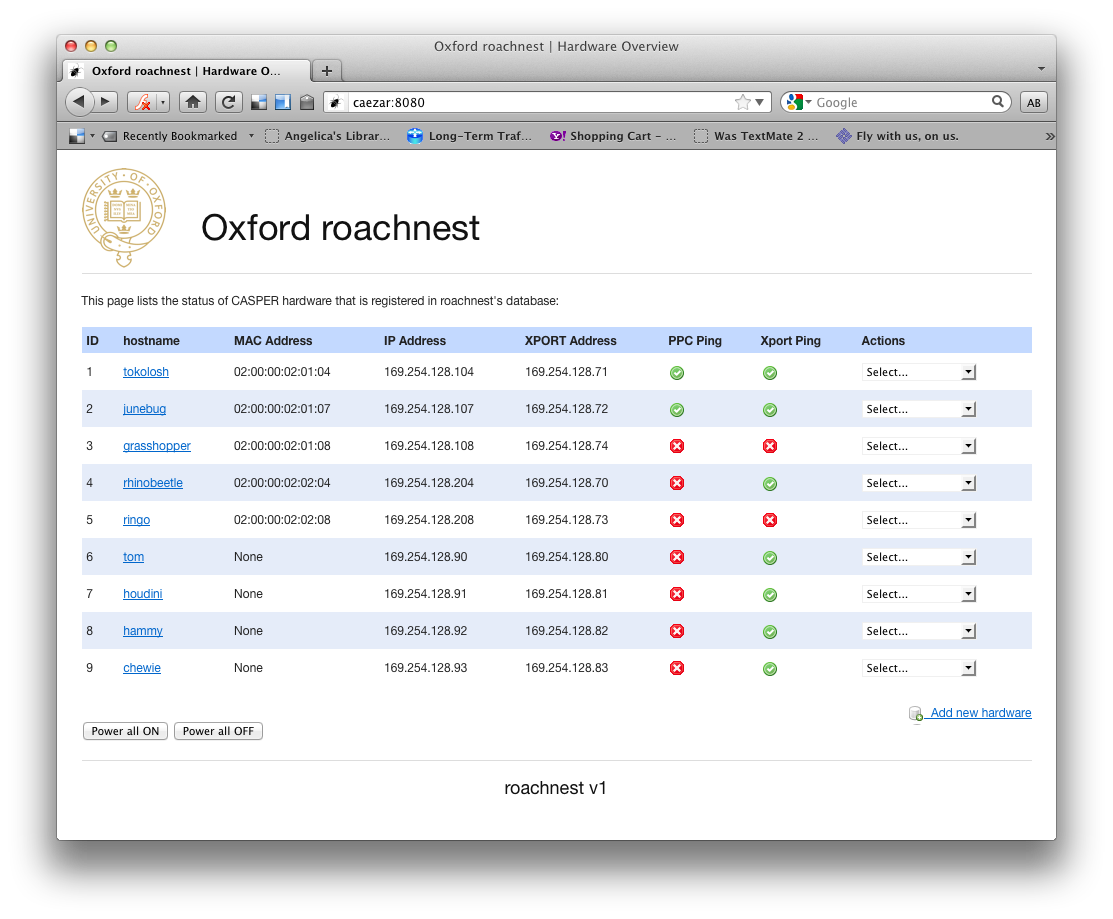
\includegraphics{screenshot_index.png}}
\caption{Homepage: hardware management}\end{figure}
\begin{figure}[htbp]
\centering
\capstart

\scalebox{0.300000}{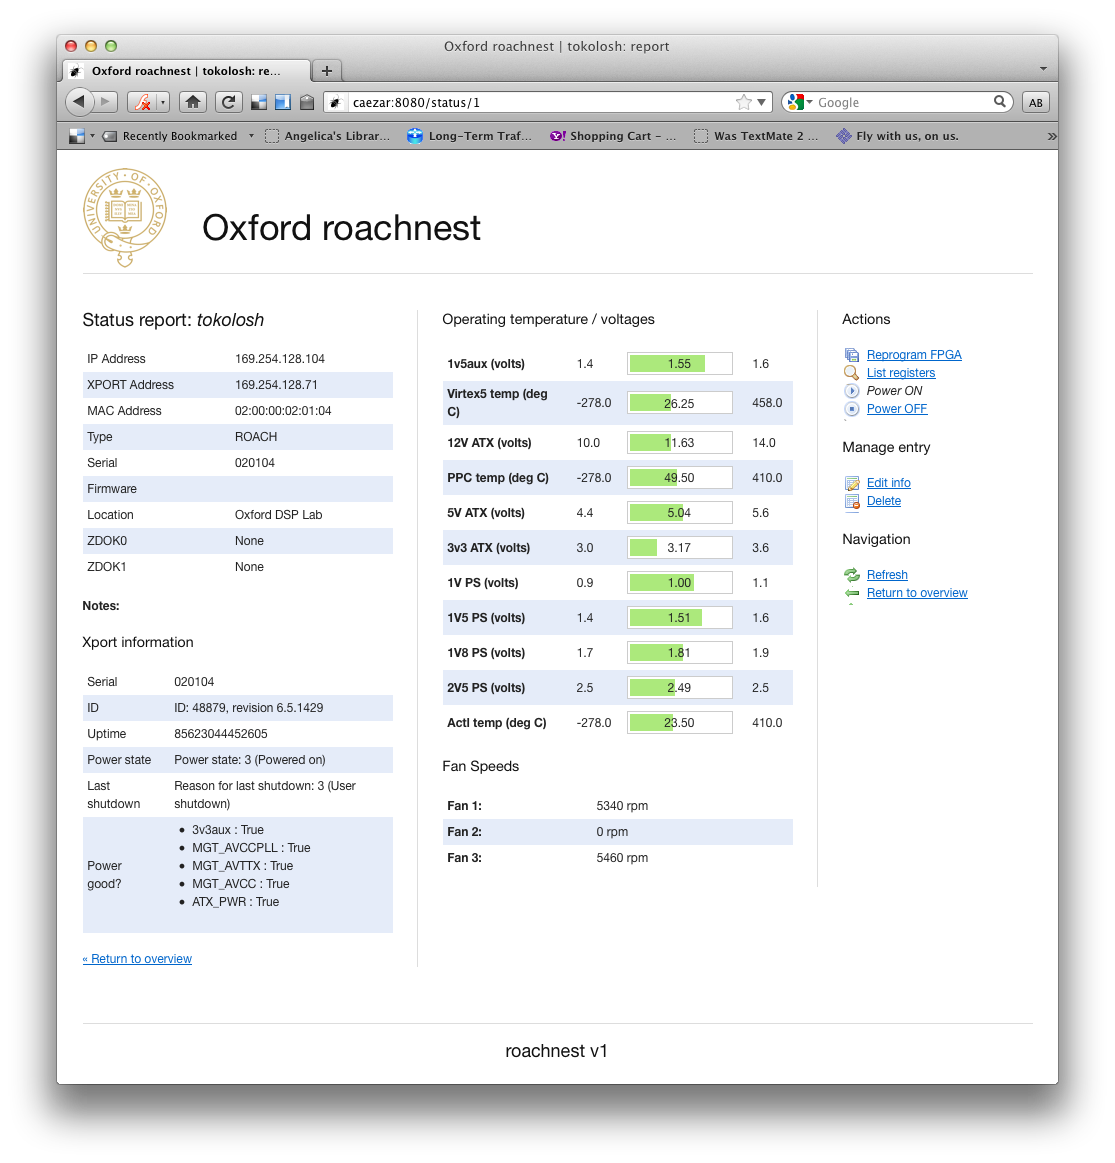
\includegraphics{screenshot_status.png}}
\caption{Detailed status and board control.}\end{figure}
\begin{figure}[htbp]
\centering
\capstart

\scalebox{0.300000}{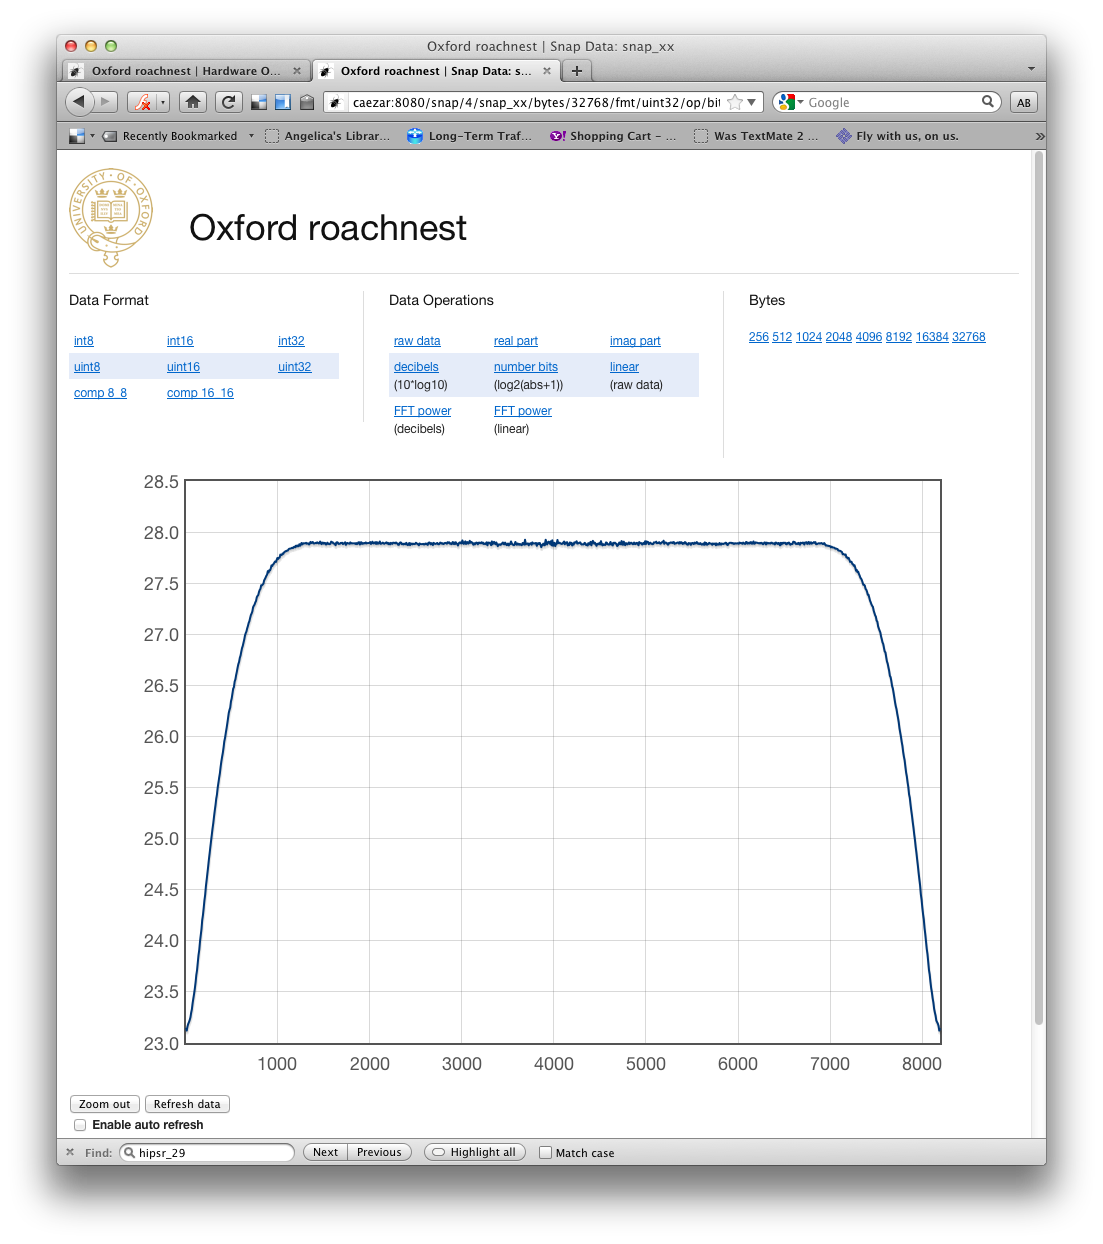
\includegraphics{screenshot_plotsnap.png}}
\caption{Javascript plotting of snap BRAMs.}\end{figure}
\begin{figure}[htbp]
\centering
\capstart

\scalebox{0.300000}{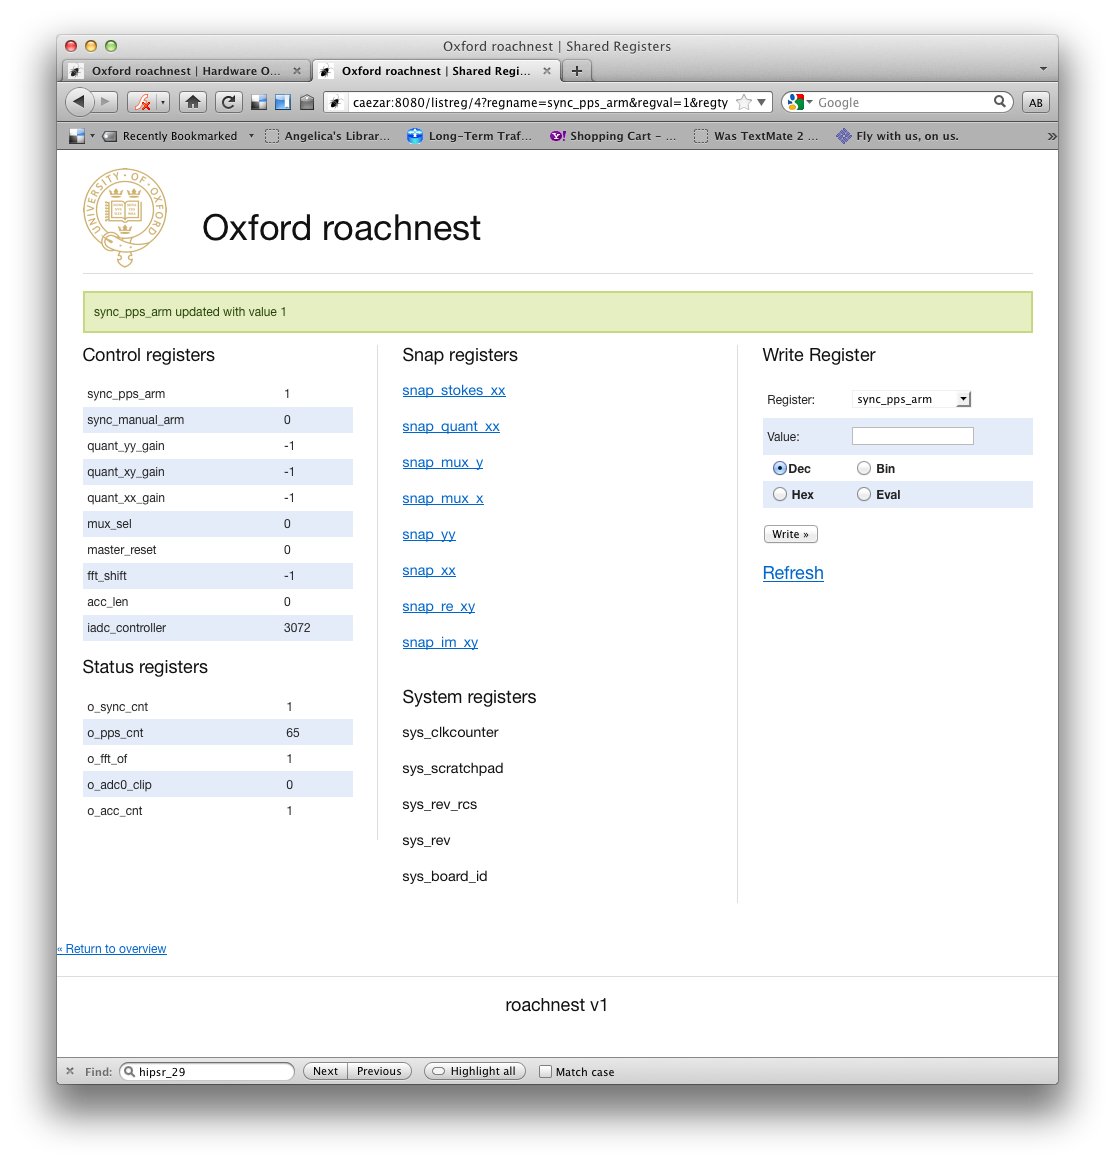
\includegraphics{screenshot_listreg.png}}
\caption{Reading and writing shared registers.}\end{figure}


\chapter{Getting Started}
\label{index:getting-started}
The first thing you'll need to do is to satisy the dependencies. You'll need:
\begin{quote}

os, sys, time, re, struct, \href{http://docs.python.org/library/sqlite3.html}{sqlite3}, \href{http://bottlepy.org/docs/dev/}{bottle}, \href{http://numpy.scipy.org/}{numpy}, \href{http://pypi.python.org/pypi/katcp/0.3.4}{katcp}, \href{http://pythonpaste.org/}{paste}, \href{http://lxml.de/}{lxml}
\end{quote}

Note that \href{http://pythonpaste.org/}{paste} and \href{http://lxml.de/}{lxml} are optional: paste improves webserver performance by using threading, and
lxml is for parsing configuration files -- although these won't appear until a future release!

After downloading the files, you should edit \emph{lib/config.py}, and check
that you're happy with the configuration. Note that you can change the page titles and the logo
in this file.

Next, assuming you've got the dependencies sorted, all you should need to do is run:

\begin{Verbatim}[commandchars=@\[\]]
@textgreater[]@textgreater[] python roachnest.py  @PYGZlb[]options@PYGZrb[]
\end{Verbatim}

This would start up a webserver on localhost:8080. The options available are:

\begin{Verbatim}[commandchars=@\[\]]
Options:
  -h, --help            show this help message and exit
  -p PORT, --port=PORT  Select KATCP port. Default is 7147
  -i HOSTIP, --hostip=HOSTIP
                        change host IP address to run server. Default is
                        localhost (127.0.0.1)
  -P HOSTPORT, --hostport=HOSTPORT
                        change host port for server. Default is 8080
\end{Verbatim}

Once the webserver is up and running, open a browser up and surf over to localhost:8080, or if you've changed
the IP address and port, type these in instead (eg. 192.168.126.6:8888). If you want the page to be viewable
over a network, you'll have to use the \emph{--hostip} option and point this to the IP address of your ethernet card.


\chapter{Module Listing}
\label{index:module-listing}\label{index:module-roachnest}
\index{roachnest (module)}

\section{roachnest.py}
\label{index:roachnest-py}
Created by Danny Price on 2011-01-12.

Copyright (c) 2011 The University of Oxford. All rights reserved.

Roachnest is a browser based Graphical User Interface (GUI) for control of CASPER hardware.
It facilitates basic monitor and control tasks, such as turning boards on and off via the XPORT, 
reprogramming the FPGA, reading and writing registers, and plotting the contents of shared BRAMS 
(snap blocks).

Roachnest also provides basic hardware management through a small sqlite database. Users can add
notes, specify IP addresses, hostnames, and other basic information necessary to keep track of
hardware specifics.

\textbf{License:} GNU GPL: \href{http://www.gnu.org/copyleft/gpl.html}{http://www.gnu.org/copyleft/gpl.html}

\textbf{Warning:} I strongly suggest that this is available only through an internal network and 
is not made accessible via the WWW. Use at your own risk.

\index{create\_db() (in module roachnest)}

\begin{fulllineitems}
\phantomsection\label{index:roachnest.create_db}\pysiglinewithargsret{\code{roachnest.}\bfcode{create\_db}}{}{}
URL: \emph{/dbcreate}

Creates a new database.

\end{fulllineitems}


\index{download() (in module roachnest)}

\begin{fulllineitems}
\phantomsection\label{index:roachnest.download}\pysiglinewithargsret{\code{roachnest.}\bfcode{download}}{\emph{filename}}{}
URL: \emph{/download/:filename}

Forces download of static files.

\end{fulllineitems}


\index{hardware\_add() (in module roachnest)}

\begin{fulllineitems}
\phantomsection\label{index:roachnest.hardware_add}\pysiglinewithargsret{\code{roachnest.}\bfcode{hardware\_add}}{}{}
URL: \emph{/add}

Add a new piece of kit to the database.

\end{fulllineitems}


\index{hardware\_edit() (in module roachnest)}

\begin{fulllineitems}
\phantomsection\label{index:roachnest.hardware_edit}\pysiglinewithargsret{\code{roachnest.}\bfcode{hardware\_edit}}{\emph{id}}{}
URL: \emph{/delete/:id}

Delete a piece of kit from the database.

\end{fulllineitems}


\index{list\_hardware() (in module roachnest)}

\begin{fulllineitems}
\phantomsection\label{index:roachnest.list_hardware}\pysiglinewithargsret{\code{roachnest.}\bfcode{list\_hardware}}{}{}
URL: \emph{/}

Index page. Lists all boards in the hardware database.

\end{fulllineitems}


\index{listbof() (in module roachnest)}

\begin{fulllineitems}
\phantomsection\label{index:roachnest.listbof}\pysiglinewithargsret{\code{roachnest.}\bfcode{listbof}}{\emph{id}}{}
URL: \emph{/listbof}

Lists all bitstreams. Uses KATCP ?listbof command.

\end{fulllineitems}


\index{listreg() (in module roachnest)}

\begin{fulllineitems}
\phantomsection\label{index:roachnest.listreg}\pysiglinewithargsret{\code{roachnest.}\bfcode{listreg}}{\emph{id}}{}
URL: \emph{/listreg}

Lists registers and applies basic sorting regex. Uses KATCP ?listdev command.

\end{fulllineitems}


\index{power\_off() (in module roachnest)}

\begin{fulllineitems}
\phantomsection\label{index:roachnest.power_off}\pysiglinewithargsret{\code{roachnest.}\bfcode{power\_off}}{\emph{id}}{}
URL: \emph{/poweroff/:id}

Powers off a ROACH board using XPORT.

\end{fulllineitems}


\index{power\_on() (in module roachnest)}

\begin{fulllineitems}
\phantomsection\label{index:roachnest.power_on}\pysiglinewithargsret{\code{roachnest.}\bfcode{power\_on}}{\emph{id}}{}
URL: \emph{/poweron/:id}

Powers up a ROACH board using XPORT.

\end{fulllineitems}


\index{progdev() (in module roachnest)}

\begin{fulllineitems}
\phantomsection\label{index:roachnest.progdev}\pysiglinewithargsret{\code{roachnest.}\bfcode{progdev}}{\emph{id}, \emph{bitstream}}{}
URL: \emph{/progdev/:bitstream}

Executes KATCP ?progdev command to program FPGA.

\end{fulllineitems}


\index{server\_static() (in module roachnest)}

\begin{fulllineitems}
\phantomsection\label{index:roachnest.server_static}\pysiglinewithargsret{\code{roachnest.}\bfcode{server\_static}}{\emph{path}}{}
URL: \emph{/files/:path\#.+\#}

Returns static files (eg images, css, scripts, favicons).

\end{fulllineitems}


\index{snap32() (in module roachnest)}

\begin{fulllineitems}
\phantomsection\label{index:roachnest.snap32}\pysiglinewithargsret{\code{roachnest.}\bfcode{snap32}}{\emph{id}, \emph{snap\_id}, \emph{bytes}, \emph{fmt}, \emph{op}}{}
URL: \emph{ajax\_snap/:snap\_id/bytes/:bytes/fmt/:fmt}

AJAX request handler for /snap plotting page. Returns JSON data for
the Flot javascript plotting library to plot.

\end{fulllineitems}


\index{view\_hardware() (in module roachnest)}

\begin{fulllineitems}
\phantomsection\label{index:roachnest.view_hardware}\pysiglinewithargsret{\code{roachnest.}\bfcode{view\_hardware}}{\emph{id}}{}
URL: \emph{/status/:id}

Provides overview of a single piece of kit.

\end{fulllineitems}

\phantomsection\label{index:module-roachnest_helpers}
\index{roachnest\_helpers (module)}

\section{roachnest\_helpers.py}
\label{index:roachnest-helpers-py}
Created by Danny Price on 2011-01-12.

Copyright (c) 2011 The University of Oxford. All rights reserved.

Helper functions and classes for roachnest.

\index{bin2dec() (in module roachnest\_helpers)}

\begin{fulllineitems}
\phantomsection\label{index:roachnest_helpers.bin2dec}\pysiglinewithargsret{\code{roachnest\_helpers.}\bfcode{bin2dec}}{\emph{binary}}{}
return the decimal string representation of \emph{binary}
\begin{quote}\begin{description}
\item[{Parameters }] \leavevmode
\textbf{binary: binary string} :
\begin{quote}

binary string to reinterpret as decimal
\end{quote}

\end{description}\end{quote}

\end{fulllineitems}


\index{dbadd() (in module roachnest\_helpers)}

\begin{fulllineitems}
\phantomsection\label{index:roachnest_helpers.dbadd}\pysiglinewithargsret{\code{roachnest\_helpers.}\bfcode{dbadd}}{\emph{hostname}, \emph{MAC\_address}, \emph{IP\_address}, \emph{location}, \emph{notes}, \emph{serial}, \emph{firmware}, \emph{atype}, \emph{XPORT\_address}, \emph{ZDOK0}, \emph{ZDOK1}}{}
Add a new piece of hardware to the database
\begin{quote}\begin{description}
\item[{Parameters }] \leavevmode
\textbf{hostname: string} :
\begin{quote}

Hostname of piece of hardware
\end{quote}

\textbf{MAC\_address: string} :
\begin{quote}

MAC address of KATCP interface
\end{quote}

\textbf{IP\_address: string} :
\begin{quote}

IP address of KATCP interface.
\end{quote}

\textbf{location: string} :
\begin{quote}

Physical location of the hardware (eg Oxford DSP lab)
\end{quote}

\textbf{notes: string} :
\begin{quote}

Any relevant notes that you may have
\end{quote}

\textbf{serial: string} :
\begin{quote}

The serial number of the hardware.
\end{quote}

\textbf{firmware:} :
\begin{quote}

Firmware revision information
\end{quote}

\textbf{atype: string} :
\begin{quote}

What type of hardware is it? Options are generally ROACH, ROACH2, iBOB or BEE2
\end{quote}

\textbf{XPORT\_address: string} :
\begin{quote}

IP address of XPORT interface.
\end{quote}

\textbf{ZDOK0: string} :
\begin{quote}

Notes about what is installed in ZDOK 0.
\end{quote}

\textbf{ZDOK1: string} :
\begin{quote}

Notes about what is installed in ZDOK 1.
\end{quote}

\end{description}\end{quote}

\end{fulllineitems}


\index{dbblank() (in module roachnest\_helpers)}

\begin{fulllineitems}
\phantomsection\label{index:roachnest_helpers.dbblank}\pysiglinewithargsret{\code{roachnest\_helpers.}\bfcode{dbblank}}{}{}
Returns a blank hardware dictionary.

Returns a BLANK python dictionary with the following entries:
id, hostname, MAC\_address, IP\_address, location, notes, serial, firmware, type,
XPORT\_address, ZDOK0, ZDOK1, status, XPORT\_status.

\end{fulllineitems}


\index{dbcreate() (in module roachnest\_helpers)}

\begin{fulllineitems}
\phantomsection\label{index:roachnest_helpers.dbcreate}\pysiglinewithargsret{\code{roachnest\_helpers.}\bfcode{dbcreate}}{}{}
Creates a new database.
\paragraph{Notes}

This function should only be called once, for initial database setup.

\end{fulllineitems}


\index{dbdelete() (in module roachnest\_helpers)}

\begin{fulllineitems}
\phantomsection\label{index:roachnest_helpers.dbdelete}\pysiglinewithargsret{\code{roachnest\_helpers.}\bfcode{dbdelete}}{\emph{id}}{}
Deletes a piece of hardware from the database.
\begin{quote}\begin{description}
\item[{Parameters }] \leavevmode
\textbf{id: int} :
\begin{quote}

Primary key (ID number) of record
\end{quote}

\end{description}\end{quote}

\end{fulllineitems}


\index{dbedit() (in module roachnest\_helpers)}

\begin{fulllineitems}
\phantomsection\label{index:roachnest_helpers.dbedit}\pysiglinewithargsret{\code{roachnest\_helpers.}\bfcode{dbedit}}{\emph{id}, \emph{hostname}, \emph{MAC\_address}, \emph{IP\_address}, \emph{location}, \emph{notes}, \emph{serial}, \emph{firmware}, \emph{atype}, \emph{XPORT\_address}, \emph{ZDOK0}, \emph{ZDOK1}}{}
Edit an exisiting piece of hardware in the database
\begin{quote}\begin{description}
\item[{Parameters }] \leavevmode
\textbf{id: int} :
\begin{quote}

Primary key (ID number) of record
\end{quote}

\textbf{hostname: string} :
\begin{quote}

Hostname of piece of hardware
\end{quote}

\textbf{MAC\_address: string} :
\begin{quote}

MAC address of KATCP interface
\end{quote}

\textbf{IP\_address: string} :
\begin{quote}

IP address of KATCP interface.
\end{quote}

\textbf{location: string} :
\begin{quote}

Physical location of the hardware (eg Oxford DSP lab)
\end{quote}

\textbf{notes: string} :
\begin{quote}

Any relevant notes that you may have
\end{quote}

\textbf{serial: string} :
\begin{quote}

The serial number of the hardware.
\end{quote}

\textbf{firmware:} :
\begin{quote}

Firmware revision information
\end{quote}

\textbf{atype: string} :
\begin{quote}

What type of hardware is it? Options are generally ROACH, ROACH2, iBOB or BEE2
\end{quote}

\textbf{XPORT\_address: string} :
\begin{quote}

IP address of XPORT interface.
\end{quote}

\textbf{ZDOK0: string} :
\begin{quote}

Notes about what is installed in ZDOK 0.
\end{quote}

\textbf{ZDOK1: string} :
\begin{quote}

Notes about what is installed in ZDOK 1.
\end{quote}

\end{description}\end{quote}

\end{fulllineitems}


\index{dbget() (in module roachnest\_helpers)}

\begin{fulllineitems}
\phantomsection\label{index:roachnest_helpers.dbget}\pysiglinewithargsret{\code{roachnest\_helpers.}\bfcode{dbget}}{\emph{id}}{}
Retrieves a hardware record from the hardware database.
\begin{quote}\begin{description}
\item[{Parameters }] \leavevmode
\textbf{id: integer} :
\begin{quote}

primary key (ID number) of database entry
\end{quote}

\end{description}\end{quote}
\paragraph{Notes}

Queries database and returns a python dictionary with the following entries:
id, hostname, MAC\_address, IP\_address, location, notes, serial, firmware, type,
XPORT\_address, ZDOK0, ZDOK1, status, XPORT\_status.

\end{fulllineitems}


\index{dbgetall() (in module roachnest\_helpers)}

\begin{fulllineitems}
\phantomsection\label{index:roachnest_helpers.dbgetall}\pysiglinewithargsret{\code{roachnest\_helpers.}\bfcode{dbgetall}}{}{}
Retrieves all records from the database.
\paragraph{Notes}

Retrieves all records from the database. Returns a list of python dictionaries, with
name: value pairs that correspond to database columns. Each python dictionary 
contains the following entries:
id, hostname, MAC\_address, IP\_address, location, notes, serial, firmware, type,
XPORT\_address, ZDOK0, ZDOK1, status, XPORT\_status.

\end{fulllineitems}


\index{dec2bin() (in module roachnest\_helpers)}

\begin{fulllineitems}
\phantomsection\label{index:roachnest_helpers.dec2bin}\pysiglinewithargsret{\code{roachnest\_helpers.}\bfcode{dec2bin}}{\emph{decimal}}{}
return the binary string representation of a \emph{decimal}
Parameters
----------
decimal: decimal string
\begin{quote}

decimal string to reinterpret as binary
\end{quote}

\end{fulllineitems}


\index{dec2hex() (in module roachnest\_helpers)}

\begin{fulllineitems}
\phantomsection\label{index:roachnest_helpers.dec2hex}\pysiglinewithargsret{\code{roachnest\_helpers.}\bfcode{dec2hex}}{\emph{n}}{}
return the hexadecimal string representation of integer \emph{n}
\begin{quote}\begin{description}
\item[{Parameters }] \leavevmode
\textbf{n: hexadecimal string} :
\begin{quote}

hexadecimal string to reinterpret as decimal
\end{quote}

\end{description}\end{quote}

\end{fulllineitems}


\index{hex2dec() (in module roachnest\_helpers)}

\begin{fulllineitems}
\phantomsection\label{index:roachnest_helpers.hex2dec}\pysiglinewithargsret{\code{roachnest\_helpers.}\bfcode{hex2dec}}{\emph{s}}{}
return the integer value of a hexadecimal string \emph{s}
\begin{quote}\begin{description}
\item[{Parameters }] \leavevmode
\textbf{s: decimal string} :
\begin{quote}

decimal string to reinterpret as hexadecimal
\end{quote}

\end{description}\end{quote}

\end{fulllineitems}


\index{safe\_eval() (in module roachnest\_helpers)}

\begin{fulllineitems}
\phantomsection\label{index:roachnest_helpers.safe_eval}\pysiglinewithargsret{\code{roachnest\_helpers.}\bfcode{safe\_eval}}{\emph{command}}{}
A safer version of the eval() command, using ast.literal\_eval
TODO: make this more functional, at the moment it's pretty useless.
\begin{quote}\begin{description}
\item[{Parameters }] \leavevmode
\textbf{command: string} :
\begin{quote}

command to evaluate (e.g. `2**10-1').
\end{quote}

\end{description}\end{quote}

\end{fulllineitems}


\index{writereg() (in module roachnest\_helpers)}

\begin{fulllineitems}
\phantomsection\label{index:roachnest_helpers.writereg}\pysiglinewithargsret{\code{roachnest\_helpers.}\bfcode{writereg}}{\emph{fpga}, \emph{name}, \emph{value}, \emph{base=10}}{}
Writes a value to an FPGA register. 
Very similar to fpga.write\_int, but you can specify the base (e.g. base 2 for binary)
\begin{quote}\begin{description}
\item[{Parameters }] \leavevmode
\textbf{fpga: katcp\_wrapper.FpgaClient object} :
\begin{quote}

fpga client object (which roach board to communitcate with)
\end{quote}

\textbf{name: string} :
\begin{quote}

register name
\end{quote}

\textbf{value: integer} :
\begin{quote}

value to write to register
\end{quote}

\textbf{base: int} :
\begin{quote}

base to write register. Default is 10 (decimal), but other bases may be used.
\end{quote}

\end{description}\end{quote}

\end{fulllineitems}

\phantomsection\label{index:module-ping}
\index{ping (module)}

\section{ping.py}
\label{index:ping-py}
Ping multiple hosts/ip addresses in parallel, using threading

\textbf{Credits:} Modified from script by Jose Porrua:
\href{http://www.joseporrua.com/2008/12/11/multi-threaded-ping-in-python}{http://www.joseporrua.com/2008/12/11/multi-threaded-ping-in-python}
However, this script didn't work for me out of the box so I modified it to get it running.

\index{Host (class in ping)}

\begin{fulllineitems}
\phantomsection\label{index:ping.Host}\pysiglinewithargsret{\strong{class }\code{ping.}\bfcode{Host}}{\emph{ip}}{}
Defines a host object.

Current attributes include: name, address and status.

\end{fulllineitems}


\index{execute() (in module ping)}

\begin{fulllineitems}
\phantomsection\label{index:ping.execute}\pysiglinewithargsret{\code{ping.}\bfcode{execute}}{\emph{host}}{}
Executes a ping command and sets the appropriate attribute.
\begin{quote}\begin{description}
\item[{Parameters }] \leavevmode
\textbf{host: ping.Host} :
\begin{quote}

A host object.
\end{quote}

\end{description}\end{quote}
\paragraph{Notes}

This is significantly different to Jose Porrua's original script, which will not match
ping requests on Mac OSX. TODO: Test this on Windows and modify if required.

\end{fulllineitems}


\index{ping() (in module ping)}

\begin{fulllineitems}
\phantomsection\label{index:ping.ping}\pysiglinewithargsret{\code{ping.}\bfcode{ping}}{\emph{hostname}}{}
Pings a single board
\begin{quote}\begin{description}
\item[{Parameters }] \leavevmode
\textbf{hostname: string} :
\begin{quote}

hostname or IP address of hardware to ping
\end{quote}

\end{description}\end{quote}

\end{fulllineitems}


\index{pingHosts() (in module ping)}

\begin{fulllineitems}
\phantomsection\label{index:ping.pingHosts}\pysiglinewithargsret{\code{ping.}\bfcode{pingHosts}}{\emph{hosts}}{}
Creates and starts pinging threads.
\begin{quote}\begin{description}
\item[{Parameters }] \leavevmode
\textbf{hosts: list {[}{]}} :
\begin{quote}

A list of host objects.
\end{quote}

\end{description}\end{quote}

\end{fulllineitems}


\index{printResults() (in module ping)}

\begin{fulllineitems}
\phantomsection\label{index:ping.printResults}\pysiglinewithargsret{\code{ping.}\bfcode{printResults}}{\emph{hosts}}{}
Prints a results: address  status  hostname
\begin{quote}\begin{description}
\item[{Parameters }] \leavevmode
\textbf{hosts: list {[}{]}} :
\begin{quote}

A list of ping.Host objects
\end{quote}

\end{description}\end{quote}

\end{fulllineitems}

\phantomsection\label{index:module-xport}
\index{xport (module)}

\section{xport.py}
\label{index:xport-py}
Created by Danny Price, 03 October 2011.

Based on roach\_monitor.py at:
\href{https://casper.berkeley.edu/wiki/Roach\_monitor\_and\_management\_subsystem}{https://casper.berkeley.edu/wiki/Roach\_monitor\_and\_management\_subsystem}

This module allows for communication with the ROACH X-port. 
ROACH has an onboard, fully independent management subsystem that can be accessed through the Xport. 
The X-port system monitors voltages and temperatures and will shut down the board 
if these are out of specification. A log is kept of the shutdown cause, its value and time.

\index{Xport (class in xport)}

\begin{fulllineitems}
\phantomsection\label{index:xport.Xport}\pysiglinewithargsret{\strong{class }\code{xport.}\bfcode{Xport}}{\emph{ip}, \emph{port}}{}
Actel Fusion X-port class, for communicating with M\&C
\paragraph{Methods}

\index{clear\_crashlog() (xport.Xport method)}

\begin{fulllineitems}
\phantomsection\label{index:xport.Xport.clear_crashlog}\pysiglinewithargsret{\bfcode{clear\_crashlog}}{}{}
Reset crash log counter

\end{fulllineitems}


\index{close() (xport.Xport method)}

\begin{fulllineitems}
\phantomsection\label{index:xport.Xport.close}\pysiglinewithargsret{\bfcode{close}}{}{}
Close xport socket connection

\end{fulllineitems}


\index{connect() (xport.Xport method)}

\begin{fulllineitems}
\phantomsection\label{index:xport.Xport.connect}\pysiglinewithargsret{\bfcode{connect}}{}{}
Connect to xport socket

\end{fulllineitems}


\index{flush() (xport.Xport method)}

\begin{fulllineitems}
\phantomsection\label{index:xport.Xport.flush}\pysiglinewithargsret{\bfcode{flush}}{}{}
Flush receive buffer

\end{fulllineitems}


\index{get\_board\_time() (xport.Xport method)}

\begin{fulllineitems}
\phantomsection\label{index:xport.Xport.get_board_time}\pysiglinewithargsret{\bfcode{get\_board\_time}}{}{}
Check and retrieve board uptime. Returns board up time in seconds (int).

\end{fulllineitems}


\index{get\_channels() (xport.Xport method)}

\begin{fulllineitems}
\phantomsection\label{index:xport.Xport.get_channels}\pysiglinewithargsret{\bfcode{get\_channels}}{}{}
Retrieves the voltage and temperatures of the PPC, V5, PSU, and Actel chips.

Returns a list of format:
(channel name, channel state, channel min operational value, channel max operational val)

\end{fulllineitems}


\index{get\_fan\_speeds() (xport.Xport method)}

\begin{fulllineitems}
\phantomsection\label{index:xport.Xport.get_fan_speeds}\pysiglinewithargsret{\bfcode{get\_fan\_speeds}}{}{}
Check and retrieve fan speeds. Returns a list of fan speeds

\end{fulllineitems}


\index{get\_id() (xport.Xport method)}

\begin{fulllineitems}
\phantomsection\label{index:xport.Xport.get_id}\pysiglinewithargsret{\bfcode{get\_id}}{}{}
Return board ID and revision

\end{fulllineitems}


\index{get\_last\_shutdown() (xport.Xport method)}

\begin{fulllineitems}
\phantomsection\label{index:xport.Xport.get_last_shutdown}\pysiglinewithargsret{\bfcode{get\_last\_shutdown}}{}{}
Check and retrieve reason for last shutdown. Returns reason as a string

\end{fulllineitems}


\index{get\_power\_good() (xport.Xport method)}

\begin{fulllineitems}
\phantomsection\label{index:xport.Xport.get_power_good}\pysiglinewithargsret{\bfcode{get\_power\_good}}{}{}
Check and retrieve power good status of voltage regulators. Returns a list of power good signals.

\end{fulllineitems}


\index{get\_power\_state() (xport.Xport method)}

\begin{fulllineitems}
\phantomsection\label{index:xport.Xport.get_power_state}\pysiglinewithargsret{\bfcode{get\_power\_state}}{}{}
Check and retrive board power state. Returns power state as a string

\end{fulllineitems}


\index{get\_serial() (xport.Xport method)}

\begin{fulllineitems}
\phantomsection\label{index:xport.Xport.get_serial}\pysiglinewithargsret{\bfcode{get\_serial}}{}{}
Check and retrieve serial number. After first query the serial
number is stored as class variable self.serial

\end{fulllineitems}


\index{power\_down() (xport.Xport method)}

\begin{fulllineitems}
\phantomsection\label{index:xport.Xport.power_down}\pysiglinewithargsret{\bfcode{power\_down}}{}{}
Power down the ROACH

\end{fulllineitems}


\index{power\_up() (xport.Xport method)}

\begin{fulllineitems}
\phantomsection\label{index:xport.Xport.power_up}\pysiglinewithargsret{\bfcode{power\_up}}{}{}
Power up the ROACH (Wake on LAN)

\end{fulllineitems}


\index{read() (xport.Xport method)}

\begin{fulllineitems}
\phantomsection\label{index:xport.Xport.read}\pysiglinewithargsret{\bfcode{read}}{\emph{addr}}{}
Reads a 16bit value from the Fusion part through the Xport.

\end{fulllineitems}


\index{toggle\_config\_h() (xport.Xport method)}

\begin{fulllineitems}
\phantomsection\label{index:xport.Xport.toggle_config_h}\pysiglinewithargsret{\bfcode{toggle\_config\_h}}{}{}
todo: Toggle PPC EEPROM boot (config H)

\end{fulllineitems}


\index{toggle\_power\_on\_reset() (xport.Xport method)}

\begin{fulllineitems}
\phantomsection\label{index:xport.Xport.toggle_power_on_reset}\pysiglinewithargsret{\bfcode{toggle\_power\_on\_reset}}{}{}
todo: Toggle auto power-on after hard-reset.

\end{fulllineitems}


\index{warm\_rst() (xport.Xport method)}

\begin{fulllineitems}
\phantomsection\label{index:xport.Xport.warm_rst}\pysiglinewithargsret{\bfcode{warm\_rst}}{}{}
Reset ROACH, but not Actel

\end{fulllineitems}


\index{write() (xport.Xport method)}

\begin{fulllineitems}
\phantomsection\label{index:xport.Xport.write}\pysiglinewithargsret{\bfcode{write}}{\emph{addr}, \emph{value}}{}
Writes a 16bit value to the Fusion part through the Xport.

\end{fulllineitems}


\end{fulllineitems}


\index{xportError}

\begin{fulllineitems}
\phantomsection\label{index:xport.xportError}\pysiglinewithargsret{\strong{exception }\code{xport.}\bfcode{xportError}}{\emph{msg}}{}
A simple class for X-port error handling

\end{fulllineitems}



\renewcommand{\indexname}{Python Module Index}
\begin{theindex}
\def\bigletter#1{{\Large\sffamily#1}\nopagebreak\vspace{1mm}}
\bigletter{p}
\item {\texttt{ping}}, \pageref{index:module-ping}
\indexspace
\bigletter{r}
\item {\texttt{roachnest}}, \pageref{index:module-roachnest}
\item {\texttt{roachnest\_helpers}}, \pageref{index:module-roachnest_helpers}
\indexspace
\bigletter{x}
\item {\texttt{xport}}, \pageref{index:module-xport}
\end{theindex}
\renewcommand{\indexname}{Python Module Index}
\begin{theindex}
\def\bigletter#1{{\Large\sffamily#1}\nopagebreak\vspace{1mm}}
\bigletter{p}
\item {\texttt{ping}}, \pageref{index:module-ping}
\indexspace
\bigletter{r}
\item {\texttt{roachnest}}, \pageref{index:module-roachnest}
\item {\texttt{roachnest\_helpers}}, \pageref{index:module-roachnest_helpers}
\indexspace
\bigletter{x}
\item {\texttt{xport}}, \pageref{index:module-xport}
\end{theindex}

\renewcommand{\indexname}{Index}
\printindex
\end{document}
